% ŠABLONA PRO PSANÍ ZÁVĚREČNÉ STUDIJNÍ PRÁCE
%%%%%%%%%%%%%%%%%%%%%%%%%%%%%%%%%%%%%%%%%%%%
% Autor: Jakub Dokulil (kubadokulil99@gmail.com)
% Tato šablona byla vytvořena tak, aby pomocí ní mohli v systému LaTeX soutěžící sázet své práce a zároveň odpovídala požadavkům na formátování vyplývajícím z wordové šablony umístěné na webu soc.cz.
%
\documentclass[12pt, a4paper, twoside, openright]{report}

\usepackage[T1]{fontenc}
\usepackage[utf8]{inputenc}
\usepackage[czech]{babel}
\usepackage{lmodern}

\usepackage{tikz}

%% Nutné balíčky a nastavení
%%%%%%%%%%%%%%%%%%%%%%%%%%%%

%% Proměnné
\newcommand\obor{INFORMAČNÍ TECHNOLOGIE} %% -- napiš číslo a název tvého oboru
\newcommand\kodOboru{18-20-M/01} %% -- napiš číslo a název tvého oboru
\newcommand\zamereni{se zaměřením na programování} %% -- napiš číslo a název tvého oboru
\newcommand\skola{Střední škola průmyslová a umělecká, Opava} %% vyplň název školy
\newcommand\trida{IT4} %% vyplň jméno svého konzultanta
\newcommand\jmenoAutora{Patrik Tomaštík}  %% vyplň své jméno
\newcommand\skolniRok{2024/25} %% vyplň rok
\newcommand\datumOdevzdani{6. 1. 2025} %% vyplň rok
\newcommand\nazevPrace{Revas - Webová aplikace pro jednoduché vyrábění testů}

\title{\nazevPrace} %% -- Název tvé práce
\author{\jmenoAutora} %% -- tvé jméno
\date{\datumOdevzdani} %% -- rok, kdy píšeš SOČku

\usepackage[top=2.5cm, bottom=2.5cm, left=3.5cm, right=1.5cm]{geometry} %% nastaví okraje, left -- vnitřní okraj, right -- vnější okraj

\usepackage[czech]{babel} %% balík babel pro sazbu v češtině
\usepackage[utf8]{inputenc} %% balíky pro kódování textu
\usepackage[T1]{fontenc}
\usepackage{cmap} %% balíček zajišťující, že vytvořené PDF bude prohledávatelné a kopírovatelné
\usepackage{lmodern}  % Přidáno pro lepší podporu českých znaků

\usepackage{graphicx} %% balík pro vkládání obrázků

\usepackage{subcaption} %% balíček pro vkládání podobrázků

\usepackage{hyperref} %% balíček, který v PDF vytváří odkazy

\linespread{1.25} %% řádkování
\setlength{\parskip}{0.5em} %% odsazení mezi odstavci


\usepackage[pagestyles]{titlesec} %% balíček pro úpravu stylu kapitol a sekcí

% Nastavení formátování nadpisů
\titleformat{\chapter}[hang]
  {\rmfamily\bfseries\Large}  % Zmenšeno z \LARGE na \Large
  {\thechapter}
  {1em}
  {\MakeUppercase}

\titleformat{\section}[hang]
  {\rmfamily\bfseries\large}  % Zmenšeno z \Large na \large
  {\thesection}
  {1em}
  {}

\titleformat{\subsection}[hang]
  {\rmfamily\bfseries\normalsize}  % Zmenšeno z \large na \normalsize
  {\thesubsection}
  {1em}
  {}

% Nastavení mezer před a za nadpisy
\titlespacing*{\chapter}{0pt}{-30pt}{8pt}  % Zmenšeno z 20pt na 8pt
\titlespacing*{\section}{0pt}{12pt}{4pt}   % Zmenšeno z 20pt/10pt na 12pt/4pt
\titlespacing*{\subsection}{0pt}{12pt}{4pt} % Zmenšeno z 20pt/10pt na 12pt/4pt

% Nastavení formátování pro nečíslované nadpisy
\titleformat{name=\chapter,numberless}[hang]
  {\rmfamily\bfseries\Large}
  {}
  {0pt}
  {\MakeUppercase}

\titleformat{name=\section,numberless}[hang]
  {\rmfamily\bfseries\large}  % Zmenšeno z \Large na \large
  {}
  {0pt}
  {}

% Nastavení mezer pro nečíslované nadpisy
\titlespacing*{name=\chapter,numberless}{0pt}{0pt}{8pt}  % Změněno z -30pt na 0pt pro první mezeru
\titlespacing*{name=\section,numberless}{0pt}{12pt}{4pt}   % Zmenšeno z 15pt/5pt na 12pt/4pt

% Nastavení fontu pro obsah
\renewcommand{\cfttoctitlefont}{\rmfamily\LARGE\bfseries}
\renewcommand{\cftchapfont}{\rmfamily\bfseries}
\renewcommand{\cftsecfont}{\rmfamily}
\renewcommand{\cftsubsecfont}{\rmfamily}

% Nastavení číslování pro obsah
\renewcommand{\cftchappresnum}{\rmfamily\bfseries}
\renewcommand{\cftsecpresnum}{\rmfamily}
\renewcommand{\cftsubsecpresnum}{\rmfamily}

\usepackage{tocloft} % Balíček pro přizpůsobení vzhledu obsahu
\setlength{\cftbeforechapskip}{10pt}  % Větší rozestup pro kapitoly
\setlength{\cftbeforesecskip}{3pt}   % Menší rozestup pro sekce

% Nastavení odsazení a formátování obsahu
\cftsetindents{chapter}{0em}{2.5em}
\cftsetindents{section}{2.5em}{3em}
\cftsetindents{subsection}{5.5em}{3.7em}
\renewcommand{\cftdotsep}{2} % Hustota teček
\renewcommand{\cftchapleader}{\cftdotfill{\cftdotsep}} % Tečky i pro kapitoly

\setcounter{secnumdepth}{2}
\setcounter{tocdepth}{2}
\usepackage{fancyhdr}
\pagestyle{fancy}
\renewcommand{\headrulewidth}{0.025pt}

\usepackage{booktabs}

\usepackage{url}

%% Balíčky co se můžou hodit :) 
%%%%%%%%%%%%%%%%%%%%%%%%%%%%%%%

\usepackage{pdfpages} %% Balíček umožňující vkládat stránky z PDF souborů, 

\usepackage{upgreek} %% Balíček pro sazbu stojatých řeckých písmen, třeba u jednotky mikrometr. Například stojaté mí: \upmu, stojaté pí: \uppi

\usepackage{amsmath}    %% Balíčky amsmath a amsfonts 
\usepackage{amsfonts}   %% pro sazbu matematických symbolů
\usepackage{esint}     %% pro sazbu různých integrálů (např \oiint)
\usepackage{mathrsfs}
\usepackage{helvet} % Helvet font
\usepackage{mathptmx} % Times New Roman
\usepackage{Oswald} % Oswald font


%% makra pro sazbu matematiky
\newcommand{\dif}{\mathrm{d}} %% makro pro sazbu diferenciálu, místo toho
%% abych musel psát '\mathrm{d}' mi stačí napsat '\dif' což je mnohem 
%% kratší a mohu si tak usnadnit práci

\usepackage{listings}
\usepackage{xcolor}

\renewcommand{\lstlistingname}{Kód}% Listing -> Algorithm
\renewcommand{\lstlistlistingname}{Seznam programových kódů}% List of Listings -> List of Algorithms

%% Definice 
\lstdefinelanguage{JavaScript}{
	morekeywords=[1]{break, continue, delete, else, for, function, if, in,
		new, return, this, typeof, var, void, while, with},
	% Literals, primitive types, and reference types.
	morekeywords=[2]{false, null, true, boolean, number, undefined,
		Array, Boolean, Date, Math, Number, String, Object},
	% Built-ins.
	morekeywords=[3]{eval, parseInt, parseFloat, escape, unescape},
	sensitive,
	morecomment=[s]{/*}{*/},
	morecomment=[l]//,
	morecomment=[s]{/**}{*/}, % JavaDoc style comments
	morestring=[b]',
	morestring=[b]"
}[keywords, comments, strings]


\lstdefinelanguage[ECMAScript2015]{JavaScript}[]{JavaScript}{
	morekeywords=[1]{await, async, case, catch, class, const, default, do,
		enum, export, extends, finally, from, implements, import, instanceof,
		let, static, super, switch, throw, try},
	morestring=[b]` % Interpolation strings.
}

\lstalias[]{ES6}[ECMAScript2015]{JavaScript}

% Nastavení barev
% Requires package: color.
\definecolor{mediumgray}{rgb}{0.3, 0.4, 0.4}
\definecolor{mediumblue}{rgb}{0.0, 0.0, 0.8}
\definecolor{forestgreen}{rgb}{0.13, 0.55, 0.13}
\definecolor{darkviolet}{rgb}{0.58, 0.0, 0.83}
\definecolor{royalblue}{rgb}{0.25, 0.41, 0.88}
\definecolor{crimson}{rgb}{0.86, 0.8, 0.24}

% Nastavení pro Python
\lstdefinestyle{Python}{
	language=Python,
	backgroundcolor=\color{white},
	basicstyle=\ttfamily,
	breakatwhitespace=false,
	breaklines=false,
	captionpos=b,
	columns=fullflexible,
	commentstyle=\color{mediumgray}\upshape,
	emph={},
	emphstyle=\color{crimson},
	extendedchars=true,  % requires inputenc
	fontadjust=true,
	frame=single,
	identifierstyle=\color{black},
	keepspaces=true,
	keywordstyle=\color{mediumblue},
	keywordstyle={[2]\color{darkviolet}},
	keywordstyle={[3]\color{royalblue}},
	literate=%
	{á}{{\'a}}1 {č}{{\v{c}}}1 {ď}{{\v{d}}}1 {é}{{\'e}}1 {ě}{{\v{e}}}1
	{í}{{\'i}}1 {ň}{{\v{n}}}1 {ó}{{\'o}}1 {ř}{{\v{r}}}1 {š}{{\v{s}}}1
	{ť}{{\v{t}}}1 {ú}{{\'u}}1 {ů}{{\r{u}}}1 {ý}{{\'y}}1 {ž}{{\v{z}}}1,		
	numbers=left,
	numbersep=5pt,
	numberstyle=\tiny\color{black},
	rulecolor=\color{black},
	showlines=true,
	showspaces=false,
	showstringspaces=false,
	showtabs=false,
	stringstyle=\color{forestgreen},
	tabsize=2,
	title=\lstname,
	upquote=true  % requires textcomp	
}


\lstdefinestyle{JSES6Base}{
	backgroundcolor=\color{white},
	basicstyle=\ttfamily,
	breakatwhitespace=false,
	breaklines=false,
	captionpos=b,
	columns=fullflexible,
	commentstyle=\color{mediumgray}\upshape,
	emph={},
	emphstyle=\color{crimson},
	extendedchars=true,  % requires inputenc
	fontadjust=true,
	frame=single,
	identifierstyle=\color{black},
	keepspaces=true,
	keywordstyle=\color{mediumblue},
	keywordstyle={[2]\color{darkviolet}},
	keywordstyle={[3]\color{royalblue}},
 literate=%
{á}{{\'a}}1 {č}{{\v{c}}}1 {ď}{{\v{d}}}1 {é}{{\'e}}1 {ě}{{\v{e}}}1
{í}{{\'i}}1 {ň}{{\v{n}}}1 {ó}{{\'o}}1 {ř}{{\v{r}}}1 {š}{{\v{s}}}1
{ť}{{\v{t}}}1 {ú}{{\'u}}1 {ů}{{\r{u}}}1 {ý}{{\'y}}1 {ž}{{\v{z}}}1,		
	numbers=left,
	numbersep=5pt,
	numberstyle=\tiny\color{black},
	rulecolor=\color{black},
	showlines=true,
	showspaces=false,
	showstringspaces=false,
	showtabs=false,
	stringstyle=\color{forestgreen},
	tabsize=2,
	title=\lstname,
	upquote=true  % requires textcomp
}

\lstdefinestyle{JavaScript}{
	language=JavaScript,
	style=JSES6Base,
}
\lstdefinestyle{ES6}{
	language=ES6,
	style=JSES6Base
}


%% Bordel pro práci - můžeš smáznout :) 
%%%%%%%%%%%%%%%%%%%

\usepackage{lipsum} %% balíček který píše lipsum (nesmyslný text, který se používá pro kontrolu typografie)

%% Začátek dokumentu
%%%%%%%%%%%%%%%%%%%%
\begin{document}
	
	\pagestyle{empty}
	\pagenumbering{arabic}
	
	\cleardoublepage

%% Titulní stránka s informacemi
%%%%%%%%%%%%%%%%%%%%%%%%%%%%%%%%%%%%%%%%
	
	{\fontfamily{phv}\selectfont
		%% Logo školy
		\begin{figure}[h]
			\centering
			
\includegraphics[width=0.6\linewidth]{skola-logo.png}
		\end{figure}
		
		
		%% Hlavička práce a její název (viz proměnná \nazev prace)
		%% \sffamily %%% bezpatkové písmo - sans serif
		{\bfseries %%% písmo na stránce je tučně
			\begin{center}
				\vspace{0.025 \textheight}
				\LARGE{ZÁVĚREČNÁ STUDIJNÍ PRÁCE}\\
				\large{dokumentace}\\
				\vspace{0.075 \textheight}
				\LARGE {\nazevPrace}\\
			\end{center}  
		}%%%
		
		\begin{figure}[h]
			\centering
			
\includegraphics[width=0.5\linewidth]{logoRevas.png}
			\label{fig:main-screen}
		\end{figure}
		
		\vspace{0.02 \textheight}
		\begin{table}[h!]
			\begin{tabular}{ll}
				\textbf{Autor:} & \jmenoAutora\\ 
				\textbf{Obor:} & \kodOboru { } \obor\\
				\textbf{} & \zamereni\\
				\textbf{Třída:} & \trida\\
				\textbf{Školní rok:} & \skolniRok\\
			\end{tabular}
			
		\end{table}		
	}
	
\cleardoublepage %% Zalomení dvojstránky
	
	\tableofcontents
	\cleardoublepage

%% Stránka obsahující poděkování a prohlášení
%%%%%%%%%%%%%%%%%%%%%%%%%%%%%%%%%%%%%%%%%%%%%%%%%%%%%%%%

%% Poděkování - nepovinné
%%%%%%%%%%%%%%%%%%%%%%%%%%%%
	
	\noindent{\large{\bfseries{Poděkování}\\}}
	\noindent Děkuji panu učiteli Mgr. Markovi Lucnemu a Ing. Petru Grussmanovi za rady při vytváření tohoto projektu.
	
	\vspace*{0.7\textheight} %% Vertikální mezeru je možné upravit

%% Prohlášení - povinné
%%%%%%%%%%%%%%%%%%%%%%%%%%%%
	\noindent{\large{\bfseries{Prohlášení}\\}}  %% uprav si koncovky podle toho na jaký rod se cítíš, vypadá to pak lépe :) 
	\noindent{Prohlašuji, že jsem závěrečnou práci vypracoval samostatně a uvedl veškeré použité 
		informační zdroje.\\}
	\noindent{Souhlasím, aby tato studijní práce byla použita k výukovým a prezentačním účelům na Střední průmyslové a umělecké škole v Opavě, Praskova 399/8.}
	\vfill
	\noindent{V Opavě \datumOdevzdani\\}
	\noindent
	\begin{minipage}{\linewidth}
		\hspace{9.5cm} 
		\begin{tabular}{@{}p{6cm}@{}}
			\dotfill \\
			Podpis autora
		\end{tabular}
	\end{minipage}
	
	\cleardoublepage %% Zalomení dvojstránky

%% Stránka obsahující abstrakt (anotaci)
%%%%%%%%%%%%%%%%%%%%%%%%%%%%%%%%%%%%%%%%%%%%%%%%%%%%%%%%	
%% Abstrakt v češtině
%%%%%%%%%%%%%%%%%%%%%%%%%%%%
	\noindent{\Large{\bfseries{Abstrakt}\\}}
	\addcontentsline{toc}{chapter}{Abstrakt}
	Revas je moderní webová aplikace navržená pro efektivní vytváření, správu a sdílení testů. Aplikace umožňuje uživatelům snadno vytvářet testy v různých formátech, které mohou zahrnovat různé typy otázek, jako jsou rozhodovací testy, spojovačky, psací testy, testy ano, ne a další bězné testy. Revas, ale zahrnuje aji testy, které se dají dát do podoby her neboli takzvané herní testy. Mezi ně patří například pexeso, oběšenec, snake, hra s dveřmi a mnoho dalších herních testů, které dělá z dělání testů zábavu. Dále obsahuje herní testy pro procviičování což tyhle testy se od herních moc neliší jen v tom, že se neznámkují, ale můžete v ních jen dostat body a tyhle testy se berou hlavně, proto aby si žák zabavil a při tom něco i přiučil. Revas nabízí uživatelům flexibilitu ve tvorbě testů, čímž poskytuje ideální nástroj pro různé scénáře – od vzdělávacích institucí po profesionální certifikační procesy.

	\vspace{18pt}
	\noindent{\large{\bfseries{Klíčová slova}}}

	\noindent vzdělávání, testy, vyrábění testů, herní testy, zábava, herní testy pro procvičování, procvičování

	\vspace{18pt}
	\noindent{\Large{\bfseries{Abstract}\\}}
	Revas is a modern web application designed for efficient test creation, management and sharing. The application allows users to easily create tests in various formats, which can include different types of questions, such as decision-making tests, dot-to-dot tests, writing tests, yes, no tests and other common tests. Revas also includes tests that can be put into the form of games, or so-called game tests. These include, for example, memory games, hangman, snake, the door game and many other game tests that make taking tests fun. It also includes game tests for practice, which are not much different from game tests, only that they are not marked, but you can only get points in them and these tests are mainly taken so that the student has fun and learns something at the same time. Revas offers users flexibility in test creation, thus providing an ideal tool for various scenarios - from educational institutions to professional certification processes.

	\vspace{18pt}
	\noindent{\large{\bfseries{Keywords}}}

	\noindent education, tests, test creation, game tests, entertainment, game tests for practice, practice

%% Definice příkazu pro podnadpisy v úvodu
\newcommand{\introsubheading}[1]{%
  {\noindent\textbf{\normalsize #1}\vspace{1pt}\par}%
}
\chapter*{ÚVOD}
\addcontentsline{toc}{chapter}{Úvod}

\introsubheading{Cíle projektu}
Hlavním cílem této práce je vytvořit jednoduchou apliakci pro vyrábění jednoduchýh testů, které přináši i prvky zábavy a motivaci se něco i přiučit.


\introsubheading{Představení projektu}
Revas je aplikace, která umožňuje vytváření testů a kvízů, ale i zábavných herních testů, které kombinují otázky a odpovědi s herními prvky. Tento nástroj je navržen tak, aby byl uživatelsky přívětivý a snadno použitelný, a to jak pro učitele, studenty, tak pro širokou veřejnost, která chce spojit zábavu a učení.

\introsubheading{Motivace}
Revas vznikl z potřeby zjednodušit proces tvorby testů a zároveň přidat do učení prvek zábavy. Motivací byla frustrace z tradičních a nudných způsobů hodnocení a učení. Chtěl jsem vytvořit nástroj, který by učitelům a lektorům umožnil snadno vytvářet personalizované testy, které zároveň zaujmou studenty. Spojení herních prvků, jako je Pexeso, s otázkami a odpovědmi, oběšenec nebo dokonce studenty milovaná hra snake, přináší nový, interaktivní způsob učení, který je motivující a zároveň efektivní. Takový přístup pomáhá zvýšit zájem o učivo, což je klíčové pro lepší zapamatování a pozitivní vztah k učení.

\introsubheading{Struktura aplikace}
Apliakce se skládá z přihlašovací stránky, která vám nabídne se přihlásit či zaregistrovat se do aplikace. Jak tak učiníte, tak se dostanete na hlavní stránku, na kterém se nachází kalendář se slidem, kde na každém slidu se můžete seznámit s různými druhy testů, ve kterých můžete vyrábět různé testy. Dále se můžete dostat na stránky, kde jsou nabídky pro výrobů testů, či uložené od jiných uživatelů. Nachází se zde i chat a profilová část se statistikami.



\chapter{Teoretická část}
	Testování je důležitým nástrojem nejen v oblasti vzdělávání, ale i v psychologii, medicíně a dalších oblastech, kde je třeba kvantifikovat a analyzovat různé schopnosti a stavy. Testy mohou mít formu otázek s výběrem odpovědí, esejí, úkolů nebo praktických zkoušek, přičemž volba formy závisí na cíli testování a povaze zkoumané oblasti.

\section{Historie a vznik testování}
Testování, jak ho známe dnes, má dlouhou historii, která sahá až do starověkých civilizací. Již ve starověkém Egyptě, Číně a Řecku se používaly formy testů pro výběr jednotlivců na různé pozice, například pro vojenské nebo vládní služby. V průběhu staletí se metody hodnocení vyvíjely, ale teprve na přelomu 19. a 20. století došlo k modernizaci testování díky rozvoji psychologie.

\subsection{Počátky moderního testování}
Za počátky moderního testování je považován vývoj psychometrie, tedy vědy o měření duševních schopností a charakteristik. Na konci 19. století vytvořil francouzský psycholog Alfred Binet první testy inteligence. Binetův test, známý jako Binet-Simon test, byl zaměřen na identifikaci dětí, které měly potíže se školním učením, a byl základem pro vznik dnešních IQ testů.

\subsection{Rozvoj testování ve 20. století}
V průběhu 20. století se testování stalo klíčovým nástrojem nejen ve vzdělávání, ale také v pracovních, vojenských a psychologických výzkumech. V roce 1916 byl ve Spojených státech vyvinut Stanford-Binet test, který rozšířil původní Binetův test a poskytl lepší nástroje pro měření inteligence. Tento test byl použit pro širokou škálu účelů, od školních zkoušek po výběr do armády.

Ve 20. letech 20. století začaly vznikat také první standardizované testy pro hodnocení výkonu studentů v širším měřítku. Testy byly zaměřeny na akademické dovednosti a vědomosti, například matematiku, čtení nebo gramatiku. V roce 1926 byl vyvinut test Scholastic Aptitude Test (SAT), který se stal jedním z nejznámějších a nejpoužívanějších nástrojů pro hodnocení výkonu studentů v USA.

\section{Druhy testů}
V současnosti existuje mnoho různých typů testů, které se liší jak formou, tak účelem. Některé z nejběžnějších typů testů zahrnují:

\begin{itemize}
	\item Testy s výběrem odpovědí: Nejrozšířenější formou testování. Studenti vybírají jednu nebo více odpovědí z předem daných možností.
	\item Esejové testy: Testy, které vyžadují, aby studenti napsali odpověď v textové formě. Tyto testy hodnotí schopnost kritického myšlení a organizování informací.
	\item Praktické testy: Používají se k hodnocení praktických dovedností, například při výuce technických nebo uměleckých oborů.
	\item Standardizované testy: Tyto testy mají pevně stanovený formát a jsou používány k měření výkonu studentů ve srovnání s širokou populací. Příkladem jsou SAT, ACT nebo GRE.
	\item Formativní testy: Cílem těchto testů není pouze hodnocení, ale i podpora učení. Jsou používány v průběhu vzdělávacího procesu, aby učitelé zjistili, jaký pokrok studenti dělají a kde je potřeba zlepšení.
\end{itemize}

\section{Význam testování ve vzdělávání}
Testování má v současném vzdělávacím systému mnoho funkcí. Mezi hlavní patří:

\begin{itemize}
	\item Hodnocení pokroku studentů: Testy umožňují měřit, jak dobře studenti zvládli učivo a jaký pokrok udělali během studia.
	\item Identifikace potřeb studentů: Testy mohou pomoci identifikovat studenty, kteří potřebují další podporu nebo kteří se nacházejí nad průměrem.
	\item Motivace k učení: Testování může sloužit jako motivace pro studenty, kteří se chtějí zlepšit nebo dokázat své schopnosti.
	\item Standardizace hodnocení: Standardizované testy poskytují objektivní způsob hodnocení, který umožňuje porovnávat výkon studentů na širší úrovni.
	\item Zpětná vazba pro učitele: Testy poskytují učitelům důležité informace o tom, jak efektivně vyučují a které oblasti je třeba zlepšit.
\end{itemize}

\section{Současné trendy v testování}
V současnosti se testování stále vyvíjí a přizpůsobuje novým technologiím a pedagogickým metodám. Mezi současné trendy patří:

\begin{itemize}
	\item Online testování: S nástupem digitálních technologií se testování přesunulo do online prostředí, což umožňuje flexibilitu a dostupnost testů pro širokou veřejnost.
	\item Gamifikace testů: V některých případech je testování spojeno s herními prvky, což má za cíl zvýšit motivaci a angažovanost studentů.
	\item Testování na bázi analýzy dat: Využití pokročilé analytiky a algoritmů k hodnocení výkonu studentů a přizpůsobení testů na míru.
	\item Automatizované hodnocení: Pokroky v umělé inteligenci umožnily automatizaci hodnocení testů, což zrychluje proces a zajišťuje větší objektivitu.
\end{itemize}


	Z tabulky je patrné, že každá aplikace má své silné a slabé stránky. Zatímco Anki vyniká v pokročilých funkcích a statistikách, postrádá moderní uživatelské rozhraní a gamifikační prvky. Quizlet nabízí dobrou rovnováhu mezi funkcionalitou a použitelností, ale mnoho pokročilých funkcí je dostupných pouze v placené verzi. Memrise má propracovaný systém gamifikace, ale je omezen především na jazykové učení a vyžaduje stálé připojení k internetu.

\chapter{Použité technologie}

\section{FileSaver.js (Pro ukládání testů)}
FileSaver.js je jednoduchá knihovna, která umožňuje ukládání datových souborů přímo na uživatelském zařízení. Tato funkce je užitečná zejména v situacích, kdy není k dispozici serverové řešení. Knihovna podporuje různé formáty, což usnadňuje export a správu dat.

Výhody: 
\begin{itemize}
    \item Umožňuje ukládání souborů na uživatelském zařízení bez potřeby serveru
    \item Podpora pro exportování dat do různých formátů (.txt, .json, .csv)
    \item Snadná implementace do webových aplikací
\end{itemize}

Nedostatky: 
\begin{itemize}
    \item Omezená podpora pro pokročilé operace s daty
    \item Problémy s velkými datovými sadami
    \item Závislost na prohlížeči, což může způsobovat nekompatibility
\end{itemize}

\section{XML}
Pro převod textových formátů do formátu Moodle XML byla použita technologie, která umožňuje automatizované generování testů, otázek a odpovědí pro platformu Moodle. XML je standardní formát používaný pro výměnu dat, ale může být poněkud těžkopádný pro ruční úpravy.

Hlavní výhody: 
\begin{itemize}
    \item Automatizované generování testových otázek a odpovědí
    \item Podpora různých typů otázek (výběr z více možností, textové odpovědi, přiřazování)
    \item Efektivní správa testového obsahu a jeho export na Moodle platformu
\end{itemize}

Nedostatky: 
\begin{itemize}
    \item Verbose formát (obsahuje velké množství redundantních dat)
    \item Obtížné na čtení a ruční úpravy
    \item Méně flexibilní ve srovnání s modernějšími formáty, jako je JSON
\end{itemize}

\section{kalendar.js}
Knihovna \textbf{kalendar.js} slouží k práci s kalendářními daty a správě událostí, což je užitečné například při nastavování termínů testů a jiných důležitých aktivit. Umožňuje vizualizaci dat v kalendářním formátu a nabízí základní funkce pro plánování.

Hlavní výhody: 
\begin{itemize}
    \item Jednoduchá implementace pro základní použití
    \item Možnost spravovat a zobrazovat události přímo v kalendáři
    \item Kompatibilita s jinými knihovnami pro rozšíření funkcionality
\end{itemize}

Nedostatky: 
\begin{itemize}
    \item Omezené možnosti přizpůsobení vzhledu kalendáře
    \item Komplexní scénáře plánování mohou vyžadovat další úpravy nebo integrace
    \item Závislost na externích knihovnách při pokročilém použití
\end{itemize}

\section{JSON}
JSON (JavaScript Object Notation) je lehký datový formát, který byl použit pro ukládání a přenos testových dat. Díky své jednoduché struktuře je snadno čitelný a podporovaný napříč mnoha programovacími jazyky.

Hlavní výhody: 
\begin{itemize}
    \item Jednoduchý a čitelný formát, který je snadno pochopitelný
    \item Velká podpora napříč programovacími jazyky a nástroji
    \item Kompaktnější než XML, což zlepšuje efektivitu přenosu dat
\end{itemize}

Nedostatky: 
\begin{itemize}
    \item Nevhodný pro složitější datové struktury s atributy
    \item Nepodporuje standardizované schéma jako XML
    \item Při velkých datových objemech může být méně efektivní
\end{itemize}


	

\chapter{Architektura aplikace}
	\section{Celková architektura}
	Webová aplikace se skládá několika stránek, které na sebe navazují. Mezi ně patří hlavně stránky s testy, herními testy a herní testy pro procvičování.

	\begin{figure}[h]
		\centering
		\includegraphics[width=0.92\linewidth]{rnYn.png}
		\caption{Architektura aplikace}
		\label{fig:architecture}
	\end{figure}

	Jednotlivé části aplikace
	\begin{itemize}
		\item Uvítací stránka
		\item registrační stránka
		\item Přihlšovací stránka
		\item Přihlašovací stránka přes github
		\item Hlavní stránka
            \item Stránka s testami
            \item Stránka s herními testami
            \item Stránka s herními testami pro procvičování
            \item Stránka s veřejnými testy od uživatelů
            \item Stránka s uloženými testy
            \item Zápisník
            \item Návod
            \item Chat
            \item Profil
	\end{itemize}

	\section{Datový model}
	Pro reprezentaci dat v aplikaci pro ukládání jsem použil Django.

	\begin{lstlisting}[style=Python, caption=Definice datových modelů]
# models.py
from django.contrib.auth.models import User
from django.db import models
from django.contrib.auth.models import User
from django.conf import settings
from django.contrib.auth.models import User
from django.contrib.auth.models import AbstractUser


class Message(models.Model):
    sender = models.ForeignKey(User, on_delete=models.CASCADE, 
    related_name='sent_messages')
    recipient = models.ForeignKey(User, on_delete=models.CASCADE, 
    related_name='received_messages', null=True, blank=True)
    text = models.TextField()
    timestamp = models.DateTimeField(auto_now_add=True)

    def __str__(self):
        return f"{self.sender} -> {self.recipient or 'Public'}: 
        {self.text[:30]}"


class TestType(models.Model):
    name = models.CharField(max_length=100, unique=True)
    description = models.TextField()

    def __str__(self):
        return self.name


class UserStatistics(models.Model):
    user = models.OneToOneField(User, on_delete=models.CASCADE)
    total_tests_created = models.PositiveIntegerField(default=0)
    test_statistics = models.JSONField(default=dict)

    def __str__(self):
        return f"Statistiky pro {self.user.username}"

    def update_statistics(self, test_type_name):
        # Zvětšíme počet pro daný typ testu
        if test_type_name in self.test_statistics:
            self.test_statistics[test_type_name] += 1
        else:
            self.test_statistics[test_type_name] = 1
        self.total_tests_created += 1
        self.save()

class Profile(models.Model):
    user = models.OneToOneField(User, on_delete=models.CASCADE)
    image = models.ImageField(upload_to='avatars/', null=True, blank=True)
    displayname = models.CharField(max_length=20, null=True, blank=True)
    info = models.TextField(null=True, blank=True)

class Test(models.Model):  # Zkontroluj, že třída má tento název
    title = models.CharField(max_length=100)
    description = models.TextField()

from django.db import models

class TestModel(models.Model):
    title = models.CharField(max_length=100)
    description = models.TextField()
    questions = models.TextField() 

class Question(models.Model):
    title = models.CharField(max_length=200)
    content = models.TextField()

class Comment(models.Model):
    question = models.ForeignKey(Question, related_name='comments', 
    on_delete=models.CASCADE)
    user = models.ForeignKey(User, on_delete=models.CASCADE)
    content = models.TextField()


	\end{lstlisting}

\chapter{Implementace frontendu a backendu}
	\section{Frontend implementace}
	\subsection{Uživatelské rozhraní}
	Vzhled uživatelského rozhraní je velmi důležité, protože dává první dojem ze stránky. Jako fronted jsem používat html a Django.
\begin{lstlisting}[style=Python]
<div class="container">
    <h1>Vytvoření Testu - Spojení otázek a odpovědí</h1>

    <input type="text" id="testName" placeholder="Název testu" />
    <textarea id="testDescription" placeholder="Popis testu" rows="4"></textarea>

    <!-- Nastavení bodování -->
    <h2>Bodování</h2>
    <div class="grade-settings">
        <label for="grade1">Známka 1 (minimální body):</label>
        <input type="number" id="grade1" name="grades[1]" min="1" value="90">
        <label for="grade2">Známka 2 (minimální body):</label>
        <input type="number" id="grade2" name="grades[2]" min="1" value="70">
        <label for="grade3">Známka 3 (minimální body):</label>
        <input type="number" id="grade3" name="grades[3]" min="1" value="50">
        <label for="grade4">Známka 4 (minimální body):</label>
        <input type="number" id="grade4" name="grades[4]" min="1" value="30">
        <label for="grade5">Známka 5 (minimální body):</label>
        <input type="number" id="grade5" name="grades[5]" min="1" value="0">
    </div>

    <input type="text" id="questionInput" placeholder="Zadejte otázku" />
    <input type="text" id="answerInput" placeholder="Zadejte odpověď" />
    <input type="number" id="pointsInput" placeholder="Bodová hodnota" />
    <button class="add-btn" onclick="addPair()">Přidat pár</button>

    <div id="pairsList">
        <!-- Seznam párů otázek a odpovědí -->
    </div>

    <button class="add-btn" onclick="startTest()">Vyzkoušet test</button>
    <button onclick="saveToHTML()">Uložit do HTML</button>
    <button onclick="saveToJSON()">Uložit do JSON</button>
    <button onclick="saveToXML()">Uložit do XML</button>


    <div id="testSection" style="display: none;">
        <h2>Test: Spojte správné páry</h2>
        <div id="testContent"></div>

        <button class="add-btn" onclick="checkTest()">Odeslat odpovědi</button>
        <button class="add-btn" onclick="restartTest()">Restartovat test</button>
    </div>
    

    <div id="resultSection" class="result-container" style="display: none;">
        <h3>Výsledky testu:</h3>
        <div id="resultTables"></div>
        <p id="testResult"></p>
        <p id="testGrade"></p>
    </div>

</div>
	\end{lstlisting}
	



	\section{Backend implementace}
	Backend aplikace jsem postavil na Djangu a při výrobě testů jsem použil Javascript.

	\begin{itemize}
		\item Databáze SQL (Ukládání testů a uživatelů)
		\item Django
		\item Javascript
            \item XML
            \item JSON
	\end{itemize}


	\section{Ukládání otázek do souborů}

	\begin{lstlisting}[style=Javascript]

function saveTestToJson() {
    const testName = document.getElementById('name').value;
    const testDescription = document.getElementById('description').value
    const questions = gatherQuestions();

    const testData = {
        name: testName,
        description: testDescription,
        questions: questions
    };

    const blob = new Blob([JSON.stringify(testData, null, 2)], 
    { type: 'application/json' });
    saveAs(blob, `${testName}.json`);
}
      
function saveTestToHtml() {
    const testName = document.getElementById('name').value;
    const testDescription = document.getElementById('description').value;
    const questions = gatherQuestions();

    let htmlContent = `
        <html>
            <head>
                <title>${testName}</title>
                <style>
                    body {
                        font-family: Arial, sans-serif;
                    }
                    .question {
                        margin-bottom: 20px;
                    }
                    .question label {
                        font-weight: bold;
                    }
                </style>
            </head>
            <body>
                <h1>${testName}</h1>
                <p>${testDescription}</p>
                <form id="testForm">
    `;

    // Generování otázek
    questions.forEach((question, index) => {
        htmlContent += `
            <div class="question">
                <p><strong>Otázka ${index + 1}:</strong> 
                ${question.text}</p>
                <label for="answer_${index}">Odpověď:</label>
                <input type="text" name="answer_${index}" 
                placeholder="Zadejte odpověď">
            </div>
        `;
    });

    htmlContent += `
            <button type="button" onclick="evaluateTest()">
            Vyhodnotit test</button>
            <div id="resultsContainer"></div> 
        </form>
        </body>
    </html>
    `;

    const blob = new Blob([htmlContent], { type: 'text/html' });
    saveAs(blob, `${testName}.html`);
}


function saveTest(type) {
    const testName = document.getElementById('testName').value;
    const testDescription = 
    document.getElementById('testDescription').value;
    const testImage = document.getElementById('testImage').files[0]; 
    const isPublic = (type === 'verejne_testy') ? true : false;

    const formData = new FormData();
    formData.append('name', testName);
    formData.append('description', testDescription);
    formData.append('image', testImage);
    formData.append('is_public', isPublic);

    // Odeslání dat na server pomocí AJAX
    fetch('/api/save_test/', {
        method: 'POST',
        body: formData
    })
    .then(response => response.json())
    .then(data => {
        if (data.success) {
            showModal('Úspěch', 'Test byl úspěšně uložen.');
        } else {
            showModal('Chyba', 'Nastala chyba při ukládání testu.');
        }
    })
    .catch(error => {
        showModal('Chyba', 'Došlo k chybě při komunikaci se serverem.');
    });
}

function saveTestToXml() {
    const testName = document.getElementById('name').value;
    const testDescription = 
    document.getElementById('description').value; 
    const questions = gatherQuestions();

    let xmlContent = `<?xml version="1.0" encoding="UTF-8"?>
<quiz>
    <name>${testName}</name>
    <description>${testDescription}</description>`;

    // Generování otázek
    questions.forEach((question, index) => {
        xmlContent += `
    <question type="multichoice">
        <name>
            <text>Otázka ${index + 1}</text>
        </name>
        <questiontext format="html">
            <text>${question.text}</text>
        </questiontext>
        <answer>
            <text>${question.correctAnswer}</text>
            <feedback>
                <text>Správná odpověď!</text>
            </feedback>
        </answer>
    </question>`;
    });

    xmlContent += `
</quiz>`;

    const blob = new Blob([xmlContent], { type: 'application/xml' });
    saveAs(blob, `${testName}.xml`);
}
	\end{lstlisting}

	
    \chapter{Testy}
    Zde se nacházejí klasické testy, s kterými se můžeme setkat normálně ve škole, maturitě či kvízu. Uživatel si může nastavit jméno testu, popisek, časovač, známky a hlavně otázky a odpovědi. Poté je může vyzkoušet v náhledu, kde se ukážou aji výsledky testu a jde se nakonec stáhnout do počítače ve formátu HTML, JSON a XML pro Moodle.

\section{Rozhodovací test}
	\begin{itemize}
		\item Přidání názvu testu
		\item Přidání popisku a obrázek testu.
		\item Přidání známkování
		\item Přidání časovače
            \item Přidání otázek a body.
            \item Přidávání odpovědí v podobě odpověď a zaškrtávání
            \item Náhled testu
            \item Výsledky testů v podobě celkový počet bodů, procentuálně, známka a počet špatných skoro správných a správných odpovědí
            \item Ukládání testu do formátu HTML, JSON a XML fromát Moodle
	\end{itemize}

    \begin{figure}[h]
		\centering
		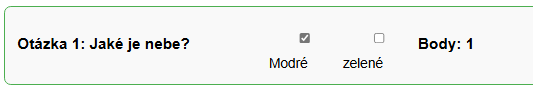
\includegraphics[width=0.8\linewidth]{fVVu.png}
		\caption{Rozhodovací test}
		\label{fig:architecture}
	\end{figure}


\section{Ano, ne test}
	\begin{itemize}
		\item Přidání názvu testu
		\item Přidání popisku a obrázek testu.
		\item Přidání známkování
		\item Přidání časovače
            \item Přidání otázek a body
            \item Přidávání odpovědí v ano, ne
            \item Náhled testu
            \item Výsledky testů v podobě celkový počet bodů, procentuálně, známka a počet špatných a správných odpovědí a vypsání správných odpovědí a označení správných
            \item Ukládání testu do formátu HTML, JSON a XML fromát Moodle
	\end{itemize}

\begin{figure}[h]
		\centering
		
\includegraphics[width=0.8\linewidth]{E8Bj.png}
		\caption{Ano, ne test}
		\label{fig:architecture}
	\end{figure}

\section{Psací test}
	\begin{itemize}
		\item Přidání názvu testu
		\item Přidání popisku a obrázek testu.
		\item Přidání známkování
		\item Přidání časovače
            \item Přidání otázek a body
            \item Přidávání odpovědí v podobě psací odpovědi
            \item Náhled testu
            \item Výsledky testů v podobě celkový počet bodů, procentuálně, známka a počet špatných a správných odpovědí a vypsání správných odpovědí a označení správných
            \item Ukládání testu do formátu HTML, JSON a XML fromát Moodle
	\end{itemize}

\begin{figure}[h]
		\centering
		
\includegraphics[width=0.8\linewidth]{ekMM.png}
		\caption{Psací test}
		\label{fig:architecture}
	\end{figure}

\section{Programovací test}
	\begin{itemize}
		\item Přidání názvu testu.
		\item Přidání popisku a obrázek testu
		\item Přidání známkování
		\item Přidání časovače
            \item Přidání otázek pro delší text a body
            \item Přidávání odpovědí v podobě delšího textu či přidání souborů
            \item Náhled testu
            \item Výsledky ukazuje jen to co uživatel vložil
            \item Ukládání testu do formátu HTML, JSON a XML fromát Moodle
	\end{itemize}

    \begin{figure}[h]
		\centering
		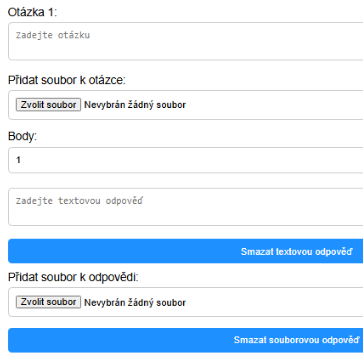
\includegraphics[width=0.3\linewidth]{RcCf.png}
		\caption{Programovací test}
		\label{fig:architecture}
	\end{figure}

    \section{Spojovací test}
	\begin{itemize}
		\item Přidání názvu testu
		\item Přidání popisku a obrázek testu.
		\item Přidání známkování
		\item Přidání časovače
            \item Přidání páru, které se mají spojit a body
            \item Náhled testu
            \item Výsledky testů v podobě celkový počet bodů, procentuálně, známka a počet špatných a správných odpovědí a vypsání správných odpovědí a označení správných
            \item Ukládání testu do formátu HTML, JSON a XML fromát Moodle
	\end{itemize}

    \begin{figure}[h]
		\centering
		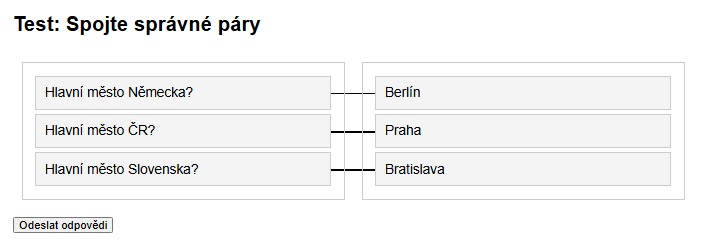
\includegraphics[width=0.8\linewidth]{GKha.png}
		\caption{Spojovací test}
		\label{fig:architecture}
	\end{figure}

    \section{tabulkový test}
	\begin{itemize}
		\item Přidání názvu testu
		\item Přidání popisku a obrázek testu.
		\item Přidání známkování
		\item Přidání časovače
            \item Přidání otázek v podobě tabulek
            \item Přidávání odpovědí v podobě odpověď do tabulky, která v ukázce se má přetáhnout
            \item Náhled testu
            \item Výsledky testů v podobě celkový počet bodů, procentuálně, známka a počet špatných a správných odpovědí a vypsání správných odpovědí a označení správných
            \item Ukládání testu do formátu HTML, JSON a XML fromát Moodle
	\end{itemize}

    \begin{figure}[h]
		\centering
		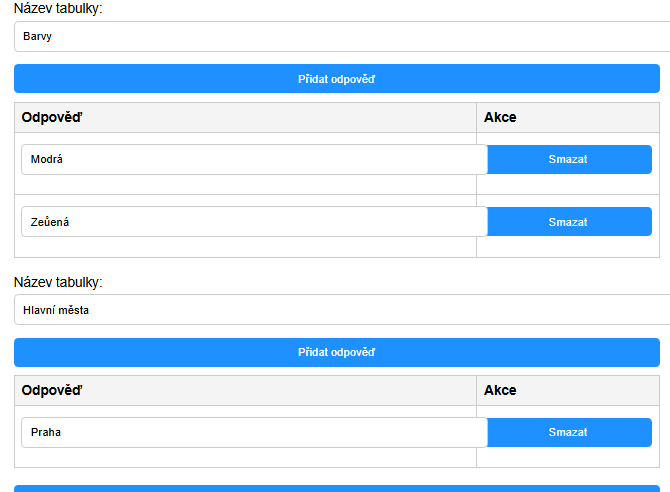
\includegraphics[width=0.8\linewidth]{NfQX.png}
            \caption{tabulkový test}
		\label{fig:architecture}
	\end{figure}

	\section{Správné odpovídací test}

	\begin{itemize}
		\item Přidání názvu testu
		\item Přidání popisku a obrázek testu.
		\item Přidání známkování
		\item Přidání časovače
            \item Přidání otázek a body
            \item Přidávání odpovědí v podobě psací odpověď a zaškrtnutí správné odpovědi
            \item Náhled testu
            \item Výsledky testů v podobě celkový počet bodů, procentuálně, známka a počet špatných a správných odpovědí a vypsání správných odpovědí a označení správných
            \item Ukládání testu do formátu HTML, JSON a XML fromát Moodle
	\end{itemize}

    \begin{figure}[h]
		\centering
		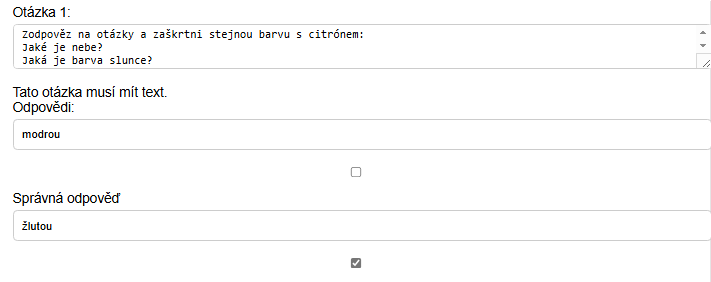
\includegraphics[width=0.8\linewidth]{rWRT.png}
		\caption{Správné odpovídací test}
		\label{fig:architecture}
	\end{figure}
		

    \chapter{Herní testy}
    Zde se nacházejí herní testy v podobě klasických a známých her. Uživatel si může nastavit jméno testu, popisek, časovač, známky a hlavně otázky a odpovědi. Poté je může vyzkoušet v náhledu, kde se ukážou aji výsledky testu a jde se nakonec stáhnout do počítače ve formátu HTML, JSON a XML pro Moodle. Každý herní test je jedinečný a zábavný. U některých testů se známky vypočítávají automaticky a nemusí se používat bodování.

\section{Pexeso}
\begin{itemize}
		\item Přidání názvu testu
		\item Přidání popisku a obrázek testu.
		\item Přidání známkování
		\item Přidání časovače
            \item Přidání párů a body
            \item Náhled testu v podobě pexesa
            \item Výsledky testů v podobě celkový počet bodů a známka
            \item Ukládání testu do formátu HTML, JSON a XML fromát Moodle
	\end{itemize}

    \begin{figure}[h]
		\centering
		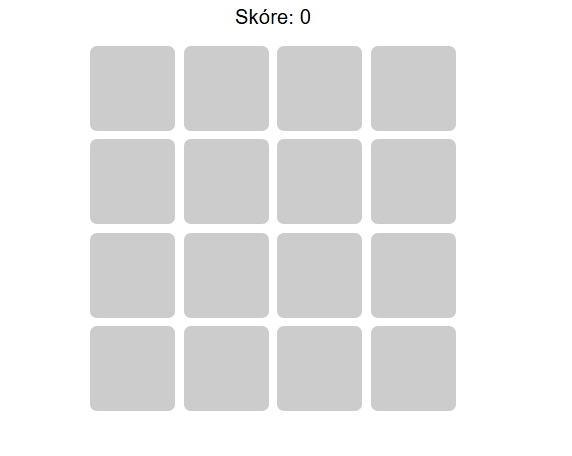
\includegraphics[width=0.4\linewidth]{dsuS.png}
		\caption{Pexeso}
		\label{fig:architecture}
	\end{figure}


\section{Oběšenec}
\begin{itemize}
		\item Přidání názvu testu
		\item Přidání popisku a obrázek testu.
		\item Přidání známkování
		\item Přidání časovače
            \item Přidání otázky a hádané odpovědi a body
            \item Náhled testu v oběšence, kde musí hádat písmena slova hádaného a má radu v podobě otázku
            ohledně toho slova. Pokud uhádne písmenko, tak zezelená, pokud ne zčervená. Má celkově 8 pokusů na uhádnutí.
            \item Výsledky testů v podobě celkový počet bodů a známka
            \item Ukládání testu do formátu HTML, JSON a XML fromát Moodle
	\end{itemize}

    \begin{figure}[h]
		\centering
		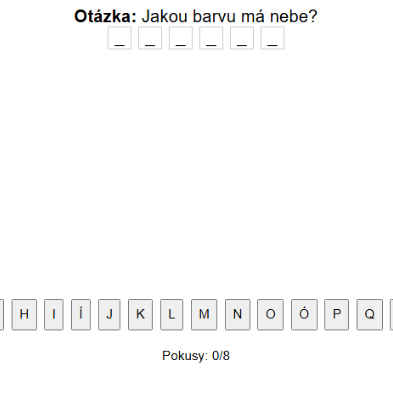
\includegraphics[width=0.8\linewidth]{SIUh.png}
		\caption{Oběšenec}
		\label{fig:architecture}
	\end{figure}

	\section{Hra s dveřmi}

\begin{itemize}
		\item Přidání názvu testu
		\item Přidání popisku a obrázek testu.
		\item Přidání známkování
		\item Přidání časovače
            \item Přidání otázky a k odpovědi a body
            \item Náhled testu v podobě, hrajeme za červenou kuličku za pomocí šipek a naším cílem je projít těmi
            správnými dveřmi. Pokažé máme otázku a každé dveře mají odpovědi, pokud projdeme správnými dveřmi, tak
            máme body pokud ne, tak nemáme body a v obou případech jdeme na další otázku pokud je. Hráč může mít navýběr i z více dveří pokud výrobce testu udělá více odpovědí, ale maximum dveří je 6.
            \item Výsledky testů v podobě celkový počet bodů a známka
            \item Ukládání testu do formátu HTML, JSON a XML fromát Moodle
	\end{itemize}

    \begin{figure}[h]
		\centering
		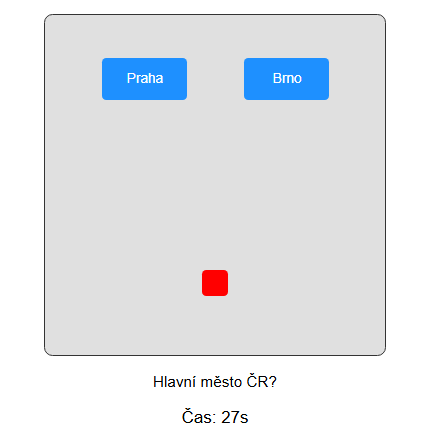
\includegraphics[width=0.5\linewidth]{m61g.png}
		\caption{Hra s dveřmi}
		\label{fig:architecture}
	\end{figure}

    \section{Snake}

\begin{itemize}
		\item Přidání názvu testu
		\item Přidání popisku a obrázek testu.
		\item Přidání známkování
		\item Přidání časovače
            \item Přidání otázky a čtyř odpovědí a body
            \item Náhled testu hry snake a nahoře se objevují otázky a odpovědi, na které musíme odpovídat přitom jak hrajeme hru snake a pokud se dotkneme zdí, tak test se ukončí a pokud odpovíme na otázku, tak po každé otázce se snake zvětšuje a nesmí se dotknout sama sebe.
            \item Výsledky testů v podobě celkový počet bodů a známka
            \item Ukládání testu do formátu HTML, JSON a XML fromát Moodle
	\end{itemize}

    \begin{figure}[h]
		\centering
		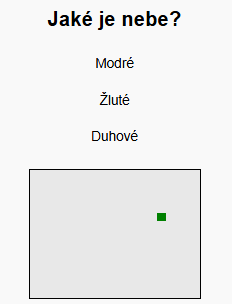
\includegraphics[width=0.3\linewidth]{LmCb.png}
		\caption{Snake}
		\label{fig:architecture}
	\end{figure}

    \section{Kámen, nůžky, papír}

\begin{itemize}
		\item Přidání názvu testu
		\item Přidání popisku a obrázek testu.
		\item Přidání známkování
		\item Přidání časovače
            \item Přidání otázek, odpovědí a nastavení pokusu hraní hry
            \item Náhled testu je jako normální testy, kde musíme klikat na správné odpovědi, ale při tom budeme mít možnost si zahrát kámen nůžky papír proti programu. Účelem je, že pokud se dostaneme na otázku, kterou opravdu nevíme a nechceme riskovat, tak můžeme si zahrát kámen nůžky papír, kde budeme muset hrát proti programu, kdo získá první tři vítězné, tak vyhrál a remízi se nepočítají. Pokud vyhraje žák, tak se mu otázka přeskočí a dá se mu za dobře a pokud vyhraje program, tak otázku přeskočí a dá se jí za špatně.
            \item Výsledky testů v podobě celkový počet bodů a známka
            \item Ukládání testu do formátu HTML, JSON a XML fromát Moodle
	\end{itemize}

    \begin{figure}[h]
		\centering
		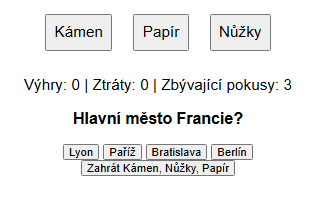
\includegraphics[width=0.5\linewidth]{f0eA.png}
		\caption{Kámen, nůžky, papír}
		\label{fig:architecture}
	\end{figure}

        \section{Maraton}

\begin{itemize}
		\item Přidání názvu testu
		\item Přidání popisku a obrázek testu.
		\item Přidání známkování
		\item Přidání časovače
            \item Přidání otázek a čtyř odpovědí, body
            \item Náhled testu, můžeme vidět našeho běžce a naším cílem je ho dostat nakonec běžecké čáry
            \item Výsledky testů v podobě celkový počet bodů a známka
            \item Ukládání testu do formátu HTML, JSON a XML fromát Moodle
	\end{itemize}

    \begin{figure}[h]
		\centering
		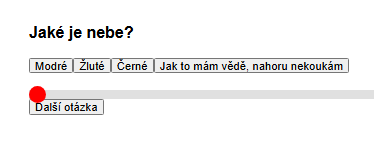
\includegraphics[width=0.4\linewidth]{Bs03.png}
		\caption{Maraton}
		\label{fig:architecture}
	\end{figure}

\chapter{Herní testy k procvičování}
 Zde se nacházejí herní testy v podobě ne moc obvyklých her. Uživatel si může nastavit jméno testu, popisek, časovač a hlavně otázky a odpovědi. Poté je může vyzkoušet v náhledu, kde se ukážou aji výsledky testu, ale jen v podobě bodech a jde se nakonec stáhnout do počítače ve formátu HTML, JSON a XML pro Moodle. Tyto testy se neznámkují, ale spíš cílem je hlavně procvičení dané látky. Každý herní test je jedinečný a zábavný.

\section{Lov pokladů}
\begin{itemize}
		\item Přidání názvu testu
		\item Přidání popisku a obrázek testu.
		\item Přidání časovače
            \item Přidání otázek a odpovědí, body
            \item Náhled testu, hrajeme za červenou kuličku, která hledá poklady. Na mapě můžeme vidět několik pokladů, ale většina je jich falešná. Pokud najdeme pravý poklad, tak nám vyskočí otázka a my musíme zodpovědět správně aby jsme dostali body. Hra končí po najití všech pokladů.
            \item Výsledky testů v podobě celkový počet bodů
            \item Ukládání testu do formátu HTML, JSON a XML fromát Moodle
	\end{itemize}

    \begin{figure}[h]
		\centering
		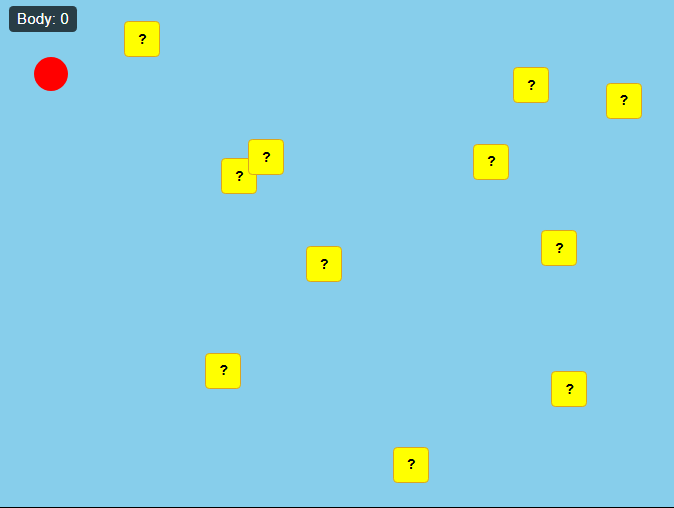
\includegraphics[width=0.5\linewidth]{iti7.png}
		\caption{Lov pokladů}
		\label{fig:architecture}
	\end{figure}


\section{Labyrint}
\begin{itemize}
		\item Přidání názvu testu
		\item Přidání popisku a obrázek testu.
		\item Přidání časovače
            \item Přidání otázek a odpovědí, body
            \item Náhled testu, Hrajeme za červenou kostku, která je vedle labyrintu, který nám pomáhá jako mapa a mi musíme poslepu získat všechny otázky v podobě kostek a dostat se do cíle co je zelený čtverec a povolí nám to ukončit jen tehdy, kdy budeme mít všechny otázky a budeme v cíly.
            \item Výsledky testů v podobě celkový počet bodů
            \item Ukládání testu do formátu HTML, JSON a XML fromát Moodle
	\end{itemize}

    \begin{figure}[h]
		\centering
		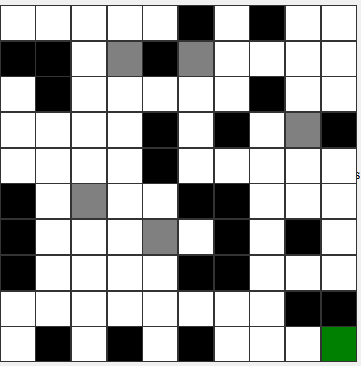
\includegraphics[width=0.5\linewidth]{28K4.png}
		\caption{Labyrint}
		\label{fig:architecture}
	\end{figure}

	\section{Flappy bird}
\begin{itemize}
		\item Přidání názvu testu
		\item Přidání popisku a obrázek testu.
		\item Přidání časovače
            \item Přidání otázek a odpovědí, body
            \item Náhled testu, klasický Flappy bird, kde musíme přeskakovat mezi trubkami a pokaždé co proskočíme trubkou, tak budeme muset odpovídat na otázky a body dostaneme jen tehdy, kdy je zodpovíme správně. Hra končí po dotknutí trubky či země.
            \item Výsledky testů v podobě celkový počet bodů
            \item Ukládání testu do formátu HTML, JSON a XML fromát Moodle
	\end{itemize}

    \begin{figure}[h]
		\centering
		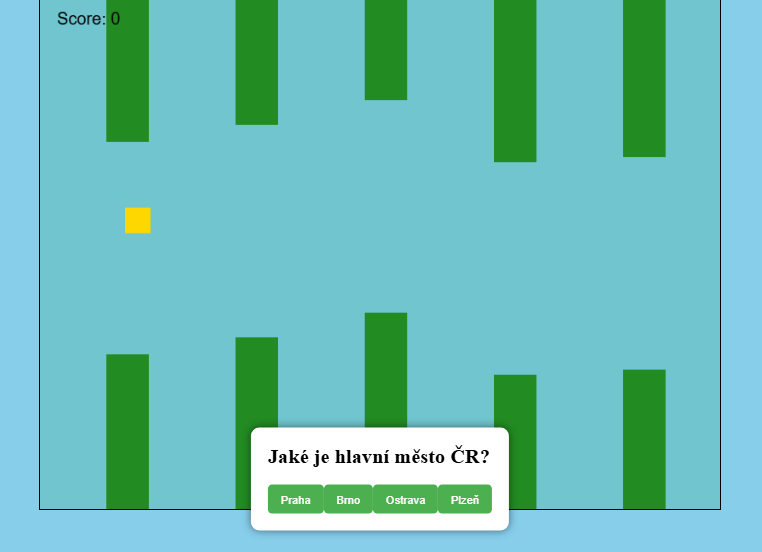
\includegraphics[width=0.8\linewidth]{6o89.png}
		\caption{Flappy bird}
		\label{fig:architecture}
	\end{figure}

    	\section{Klikačka}
\begin{itemize}
		\item Přidání názvu testu
		\item Přidání popisku a obrázek testu.
		\item Přidání časovače
            \item Přidání otázek a odpovědí, body
            \item Náhled testu, ukáže se nám otázka a odpovědi se nám náhodně ve velké rychlosti pohybují po mapě a naším cílem je chytit tu správnou odpověď. Hra končí po zodpovězení všech otázek.
            \item Výsledky testů v podobě celkový počet bodů
            \item Ukládání testu do formátu HTML, JSON a XML fromát Moodle
	\end{itemize}

    \begin{figure}[h]
		\centering
		
\includegraphics[width=0.8\linewidth]{4UWz.png}
		\caption{Klikačka}
		\label{fig:architecture}
	\end{figure}

    	\section{Miny}
\begin{itemize}
		\item Přidání názvu testu
		\item Přidání popisku a obrázek testu.
		\item Přidání časovače
            \item Přidání otázek a odpovědí, body a počet kliků
            \item Náhled testu, máme minové pole a po každém kliku se nám objeví číslo, jestli je poblíž otázka a pokud je nějaká v okolí otázka, tak ukáže počet v okolí. Pokud je to otázka a zodpovíme jí dobře, tak políčko se zbarví dozelena a máme body a pokud špatně, tak do červena a nemáme body.
            \item Výsledky testů v podobě celkový počet bodů
            \item Ukládání testu do formátu HTML, JSON a XML fromát Moodle
	\end{itemize}
  

    	\section{Tetris}

\begin{itemize}
		\item Přidání názvu testu
		\item Přidání popisku a obrázek testu.
		\item Přidání časovače
            \item Přidání otázek a odpovědí, body
            \item Náhled testu je klasický tetris, kde padají z nebe tvary a naším cílem je spojit ve řádcích. Pokud je spojíme, tak se nám ukáže otázka a pokud ji zodpovíme dobře či ne, tak podle toho dostaneme body. Vpravo se ukazují budoucí tvary a hra končí pokud nepůjdou padat další tvary.
            \item Výsledky testů v podobě celkový počet bodů
            \item Ukládání testu do formátu HTML, JSON a XML fromát Moodle
	\end{itemize}

    \begin{figure}[h]
		\centering
		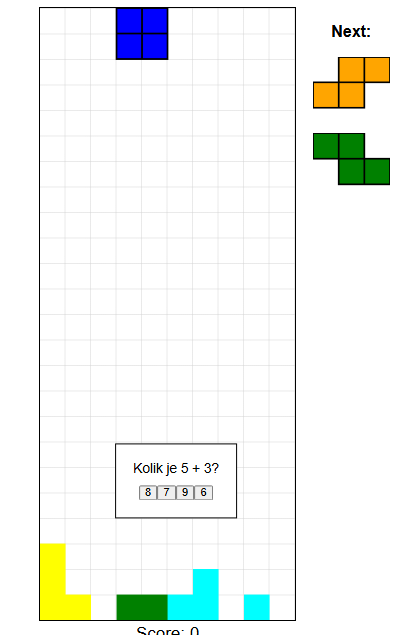
\includegraphics[width=0.4\linewidth]{kizE.png}
		\caption{Tetris}
		\label{fig:architecture}
	\end{figure}
    
    \chapter{Výsledky}

\section{Splněné cíle}
	\begin{itemize}
		\item Vyrobení jak základních, tak i testů v herní a procvičovací podobě her
		\item Základní upravování testů
		\item Přihlašování do aplikace a registrace nových uživatelů
		\item Fuunkční chat.
            \item Fuunkční ukládání testů v různých formátech do počítače a do aplikace
            \item Statistiky vyrobených testů
	\end{itemize}


\section{Nedostatky a budoucí zlepšení}
	\begin{itemize}
		\item Přidání více testů
		\item Přidání větší volnosti při vytváření testů
		\item Platby či nějaký obchod a měna, která by byla možná za odměnu vyrobeného testu
		\item Přidání dalších druhů testů v podobě kahootu a nebo denních výzev
	\end{itemize}

	\section{Přínosy}

	\begin{itemize}
	\item Efektivnější dělání testů.
        \item Zábavu
        \item Zkušenosti jak zacházet s časem a plánování
        \item Zkušenosti do budoucna
		
	\end{itemize}

    

\chapter{Závěr}
	Aplikace Revas představuje moderní nástroj, který výrazně usnadňuje tvorbu a správu testů v různých formách. Díky flexibilnímu přístupu a intuitivnímu uživatelskému rozhraní nabízí uživatelům širokou škálu možností pro tvorbu jak klasických testů, tak i v podobě her a na procvičení. Celkově jsem si tvorbu této aplikace užil. Přiučil jsem se mnoho nových věcí a osvěžil jsem si práci s Djangem a Javascriptem což jsou mé dva jazyky, které nemám moc v lásce. Nejvíce jsem si užíval dělání herních testů, kde jsem se snažil udělat klasické hry, které každý zná a rád si zahraje. Nachází se zde určitě mnoho nedostatků a věcí, kterých se dají změnit či udělat úplně jinak, ale snažil jsem se nejvíce o to aby to bylo hlavně fuunkční. Dalo mi to jak hodně zkušeností, tak hlavně poučení o tom, že toho času opravdu moc není a je opravdu důležité s ním zacházet a plánovat lépe. I přes všechny moje útrapy a nervy, které jsem stratil při dělání tohohle projekt, který jsem několikrát chtěl vzdát a dělat úplně něco jiného jsem nakonec vyrobil webovou aplikaci pro dělání testů, kde jsem si splnil nakonec i své základní cíle., Nakonec mám webovou aplikaci, na kterou můžu být hrdý, protože jsem do ní dal hodně práce a určitě v budoucnu v ní budu pokračovat.

	Zdrojový kód projektu je na GitHubu (\url{https://github.com/Patrik1T/Maturitniprojekt?tab=readme-ov-file#classquiz}).

\chapter*{Seznam použitých informačních zdrojů}
\addcontentsline{toc}{chapter}{Seznam použitých informačních zdrojů}

[1] 10.9. Quiz Flask App by simboli: Open-source webová aplikace postavená na Pythonu a Flasku s MySQL databází, umožňuje vytváření a správu kvízů. Dostupné z: \url{https://github.com/thepasterover/flask-quiz-app}

[2] 10.9. Quiz Flask App Open-source webová aplikace postavená na Pythonu a Flasku s MySQL databází, umožňuje vytváření a správu kvízů. Dostupné z: \url{https://github.com/simboli/quiz-flask-app}

[3] 10.9. ClassQuiz: Open-source aplikace podobná Kahoot!, umožňuje učitelům vytvářet kvízy, které mohou studenti hrát na dálku. 
 Dostupné z: \url{https://github.com/mawoka-myblock/ClassQuiz}

[4]9.10. Moosh: Nástroj pro správu Moodle z příkazové řádky, který může pomoci při exportu testů do Moodle. Dostupné z: \url{https://github.com/tmuras/moosh}

[5] 9.10.Moodle XML format: Nástroj pro import a export testových otázek a odpovědí do platformy Moodle ve strukturovaném XML formátu. Dostupné z: \url{https://docs.moodle.org/405/en/Moodle_XML_format}

[6] 9.10.JSON: Lehký formát pro výměnu a ukládání dat, ideální pro jednoduché a efektivní manipulace s daty mezi aplikacemi. Dostupné z: \url{https://zdrojak.cz/clanky/json-jednotny-format-pro-vymenu-dat/}

\end{document}
